\section{Filtering in the Frequency Domain}

In the unwrapped phase maps, an additional problem that needs to be resolved are the sinusoidal fringe artifacts which still remain after background subtraction and they obstruct the details in the image as well that we would want to observe. A method that can remove this is filtering in the Fourier (frequency) domain.

The concept of FFT filtering is being used extensively in image processing techniques for enhancement of wanted details or components in an image or removal of noise and unwanted frequencies \cite{Gonzalez2002}. 

Some methods of filtering and removal of noise and artifacts in PSP include the use of moving kernel filters \cite{Wang2014a}, Gaussian filters \cite{Feng2013}, or use of global phase filters \cite{Song2014}. Our method, however, uses filtering in frequency domain itself to specifically remove the fringe artifacts.

%Filtering can either be done in the space domain (image itself) or the frequency  domain. The latter is implemented by simply multiplying the image's FFT to the designed filter mask. 

FFT filtering was applied to the images by creating a filter mask concealing the unwanted frequencies in the Fourier domain which correspond to the sinusoidal fringes. The designed filter mask is then multiplied to the image's FFT. In other terms, the unwanted frequencies were removed by simply setting their corresponding pixel intensities to zero in the Fourier domain.

\section{Phase Maps After FFT Filtering}
Due to the presence of the sinusoidal fringe artifacts even with background subtraction, the processed test objects from Chapter 4 were FFT-filtered by creating filter masks for each. 

Starting with the one with the most obvious sinusoidal fringe artifacts, the styrofoam board with engraving was filtered first as shown in Figure \ref{fig:Vfft}. The FFT only operates in grayscaled images. 

\begin{figure}[h!]
	\centering
	\subfigure[]{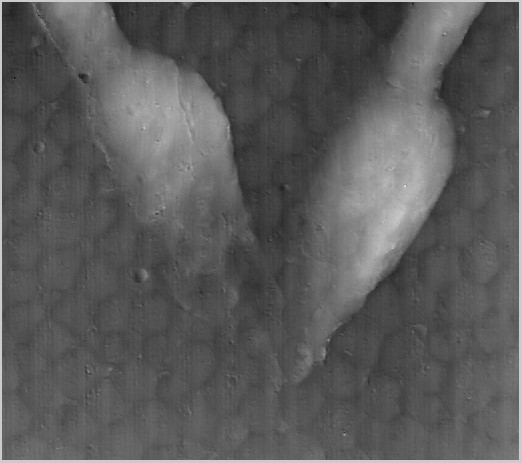
\includegraphics[width=0.34\textwidth]{figures/Vgray.jpg}\label{fig:vgray}}
	\subfigure[]{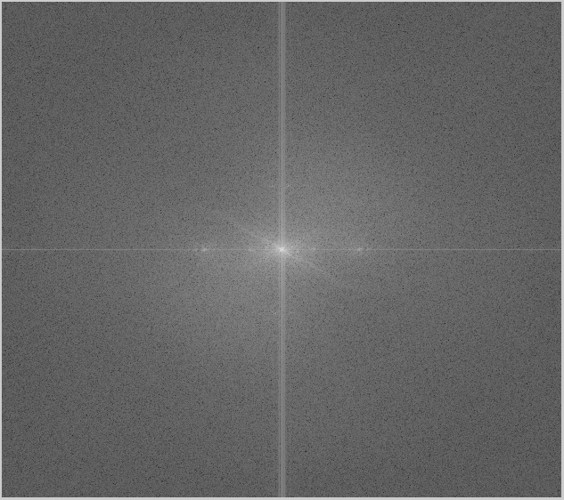
\includegraphics[width=0.34\textwidth]{figures/Vgrayfft.jpg}\label{fig:vfft}}
	\subfigure[]{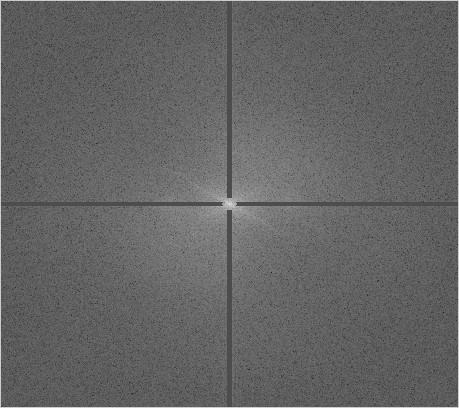
\includegraphics[width=0.34\textwidth]{figures/Vgraymask.jpg}\label{fig:vmask}}
	\subfigure[]{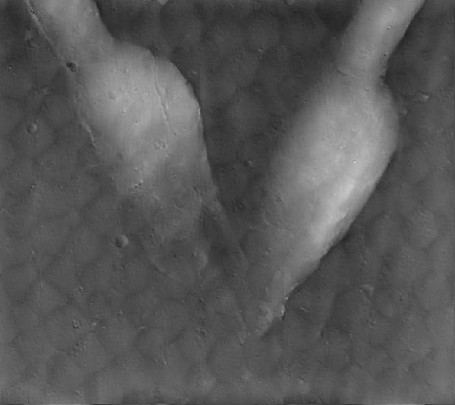
\includegraphics[width=0.34\textwidth]{figures/Vgrayfiltered.jpg}\label{fig:vfilter}}
	\caption[FFT of styrofoam board with engraving]{Styrofoam with engraving: (a) grayscaled image of the processed (without vignetting effect) unwrapped phase map, (b) FFT of the image in (a), (c) FFT filter mask, (d) phase map after applying filter mask.}
	\label{fig:Vfft}
\end{figure}

We see a cross-shaped FFT with a bright central (zero) frequency (see fig. \ref{fig:Vfft}b). 
We avoid removing the zero frequency since this contains most of the information of the image.
Also, two dominant peaks along the horizontal line which were offset from the central frequency can be observed. 
These peaks correspond to the frequency of the sinusoidal fringes that were projected to the object.
A sinusoid along the y-direction has two dirac-deltas along the x-axis for its FT \cite{Wahl1987}; hence, a verification that the fringes are still present in the phase map.

Figures \ref{fig:Vfft}c and \ref{fig:Vfft}d show the filter mask and filtered phase map of the styrofoam object, respectively. A filter mask was created masking both the horizontal and vertical frequencies since we are interested in removing the repeating fringes in the space domain. By applying the filter mask, we finally obtain an artifact-free phase map.

The transitions from the unprocessed unwrapped phase map to processed with removed vignetting effect and fringe artifacts for the styrofoam board is seen in Figure \ref{fig:Vprocessed}.

\begin{figure}[h!]
	\centering
	\subfigure[]{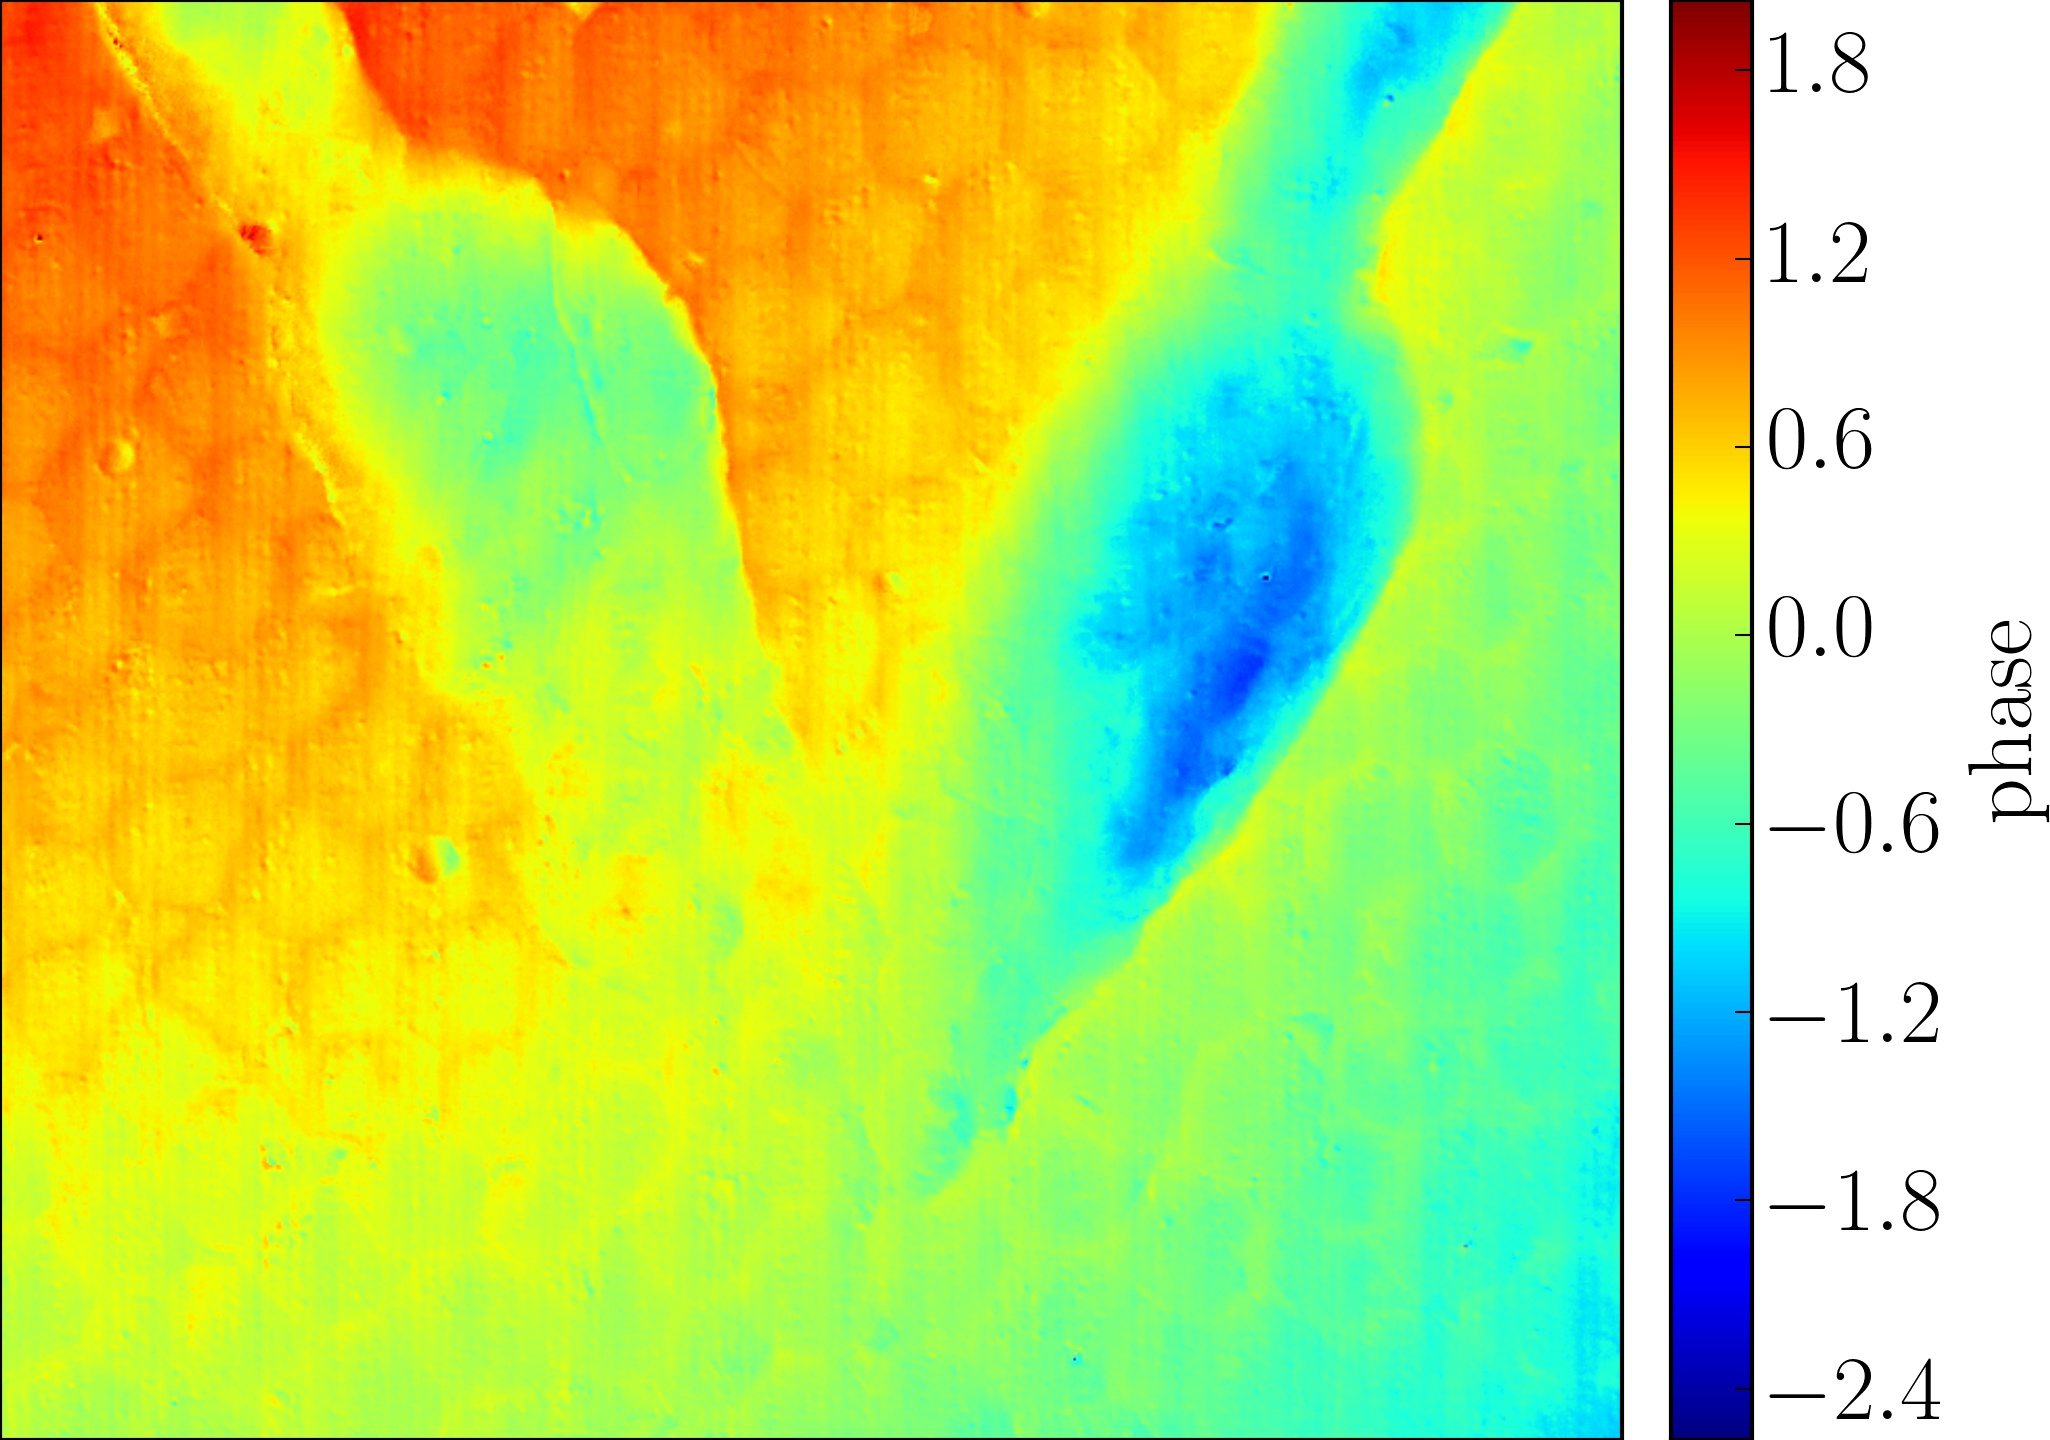
\includegraphics[width=0.4\textwidth]{figures/V.jpg}}
	\subfigure[]{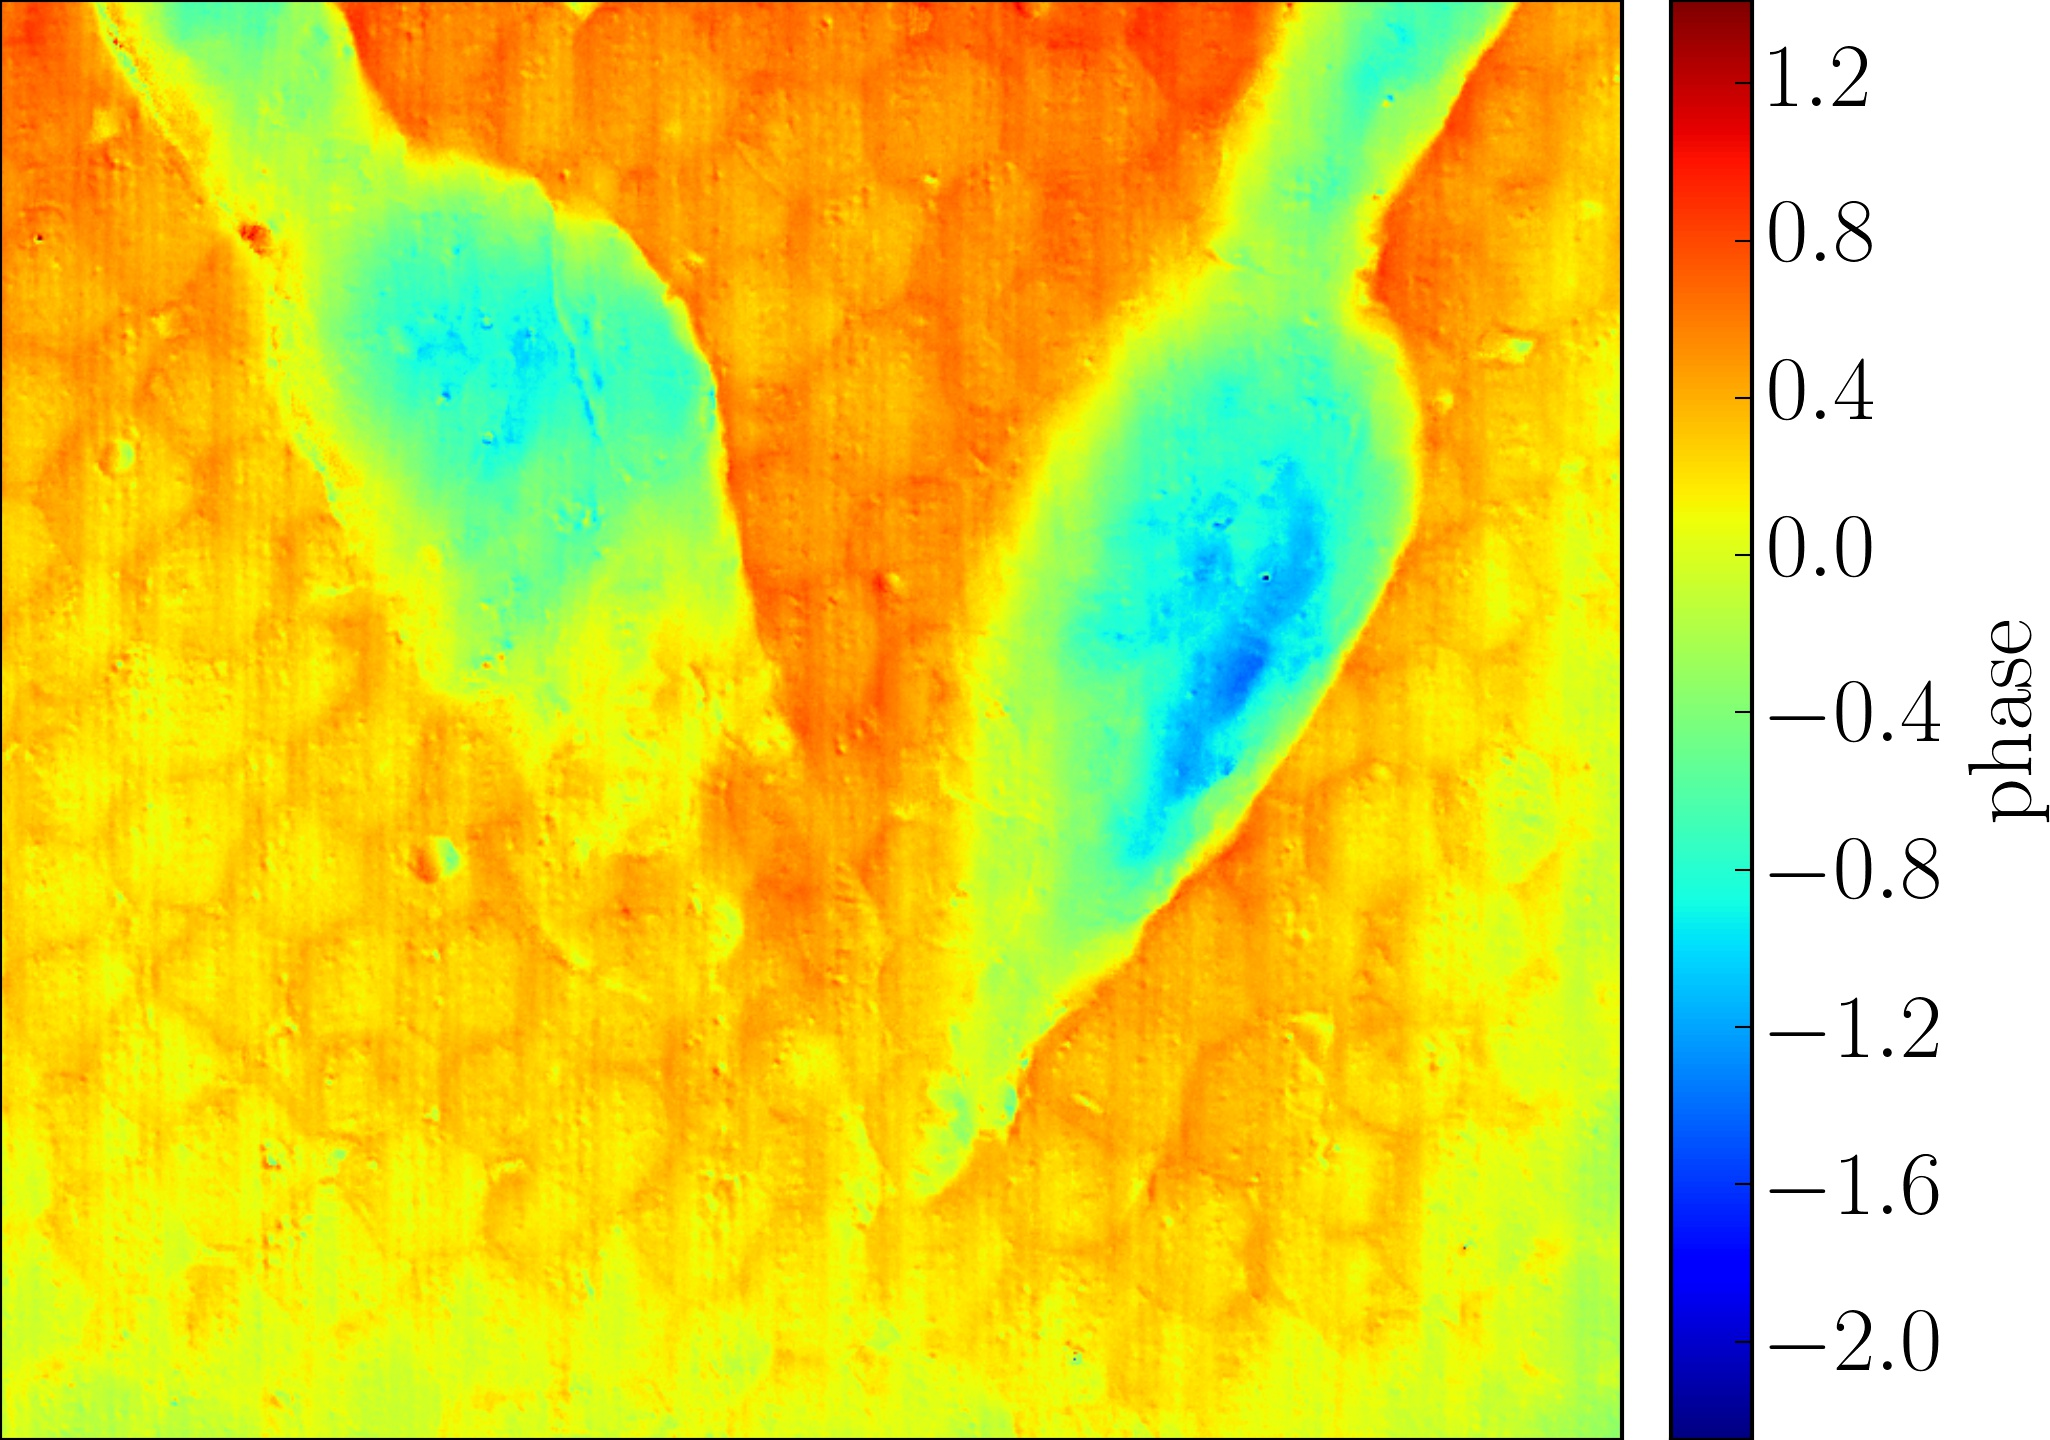
\includegraphics[width=0.4\textwidth]{figures/V_BS.jpg}}
	\subfigure[]{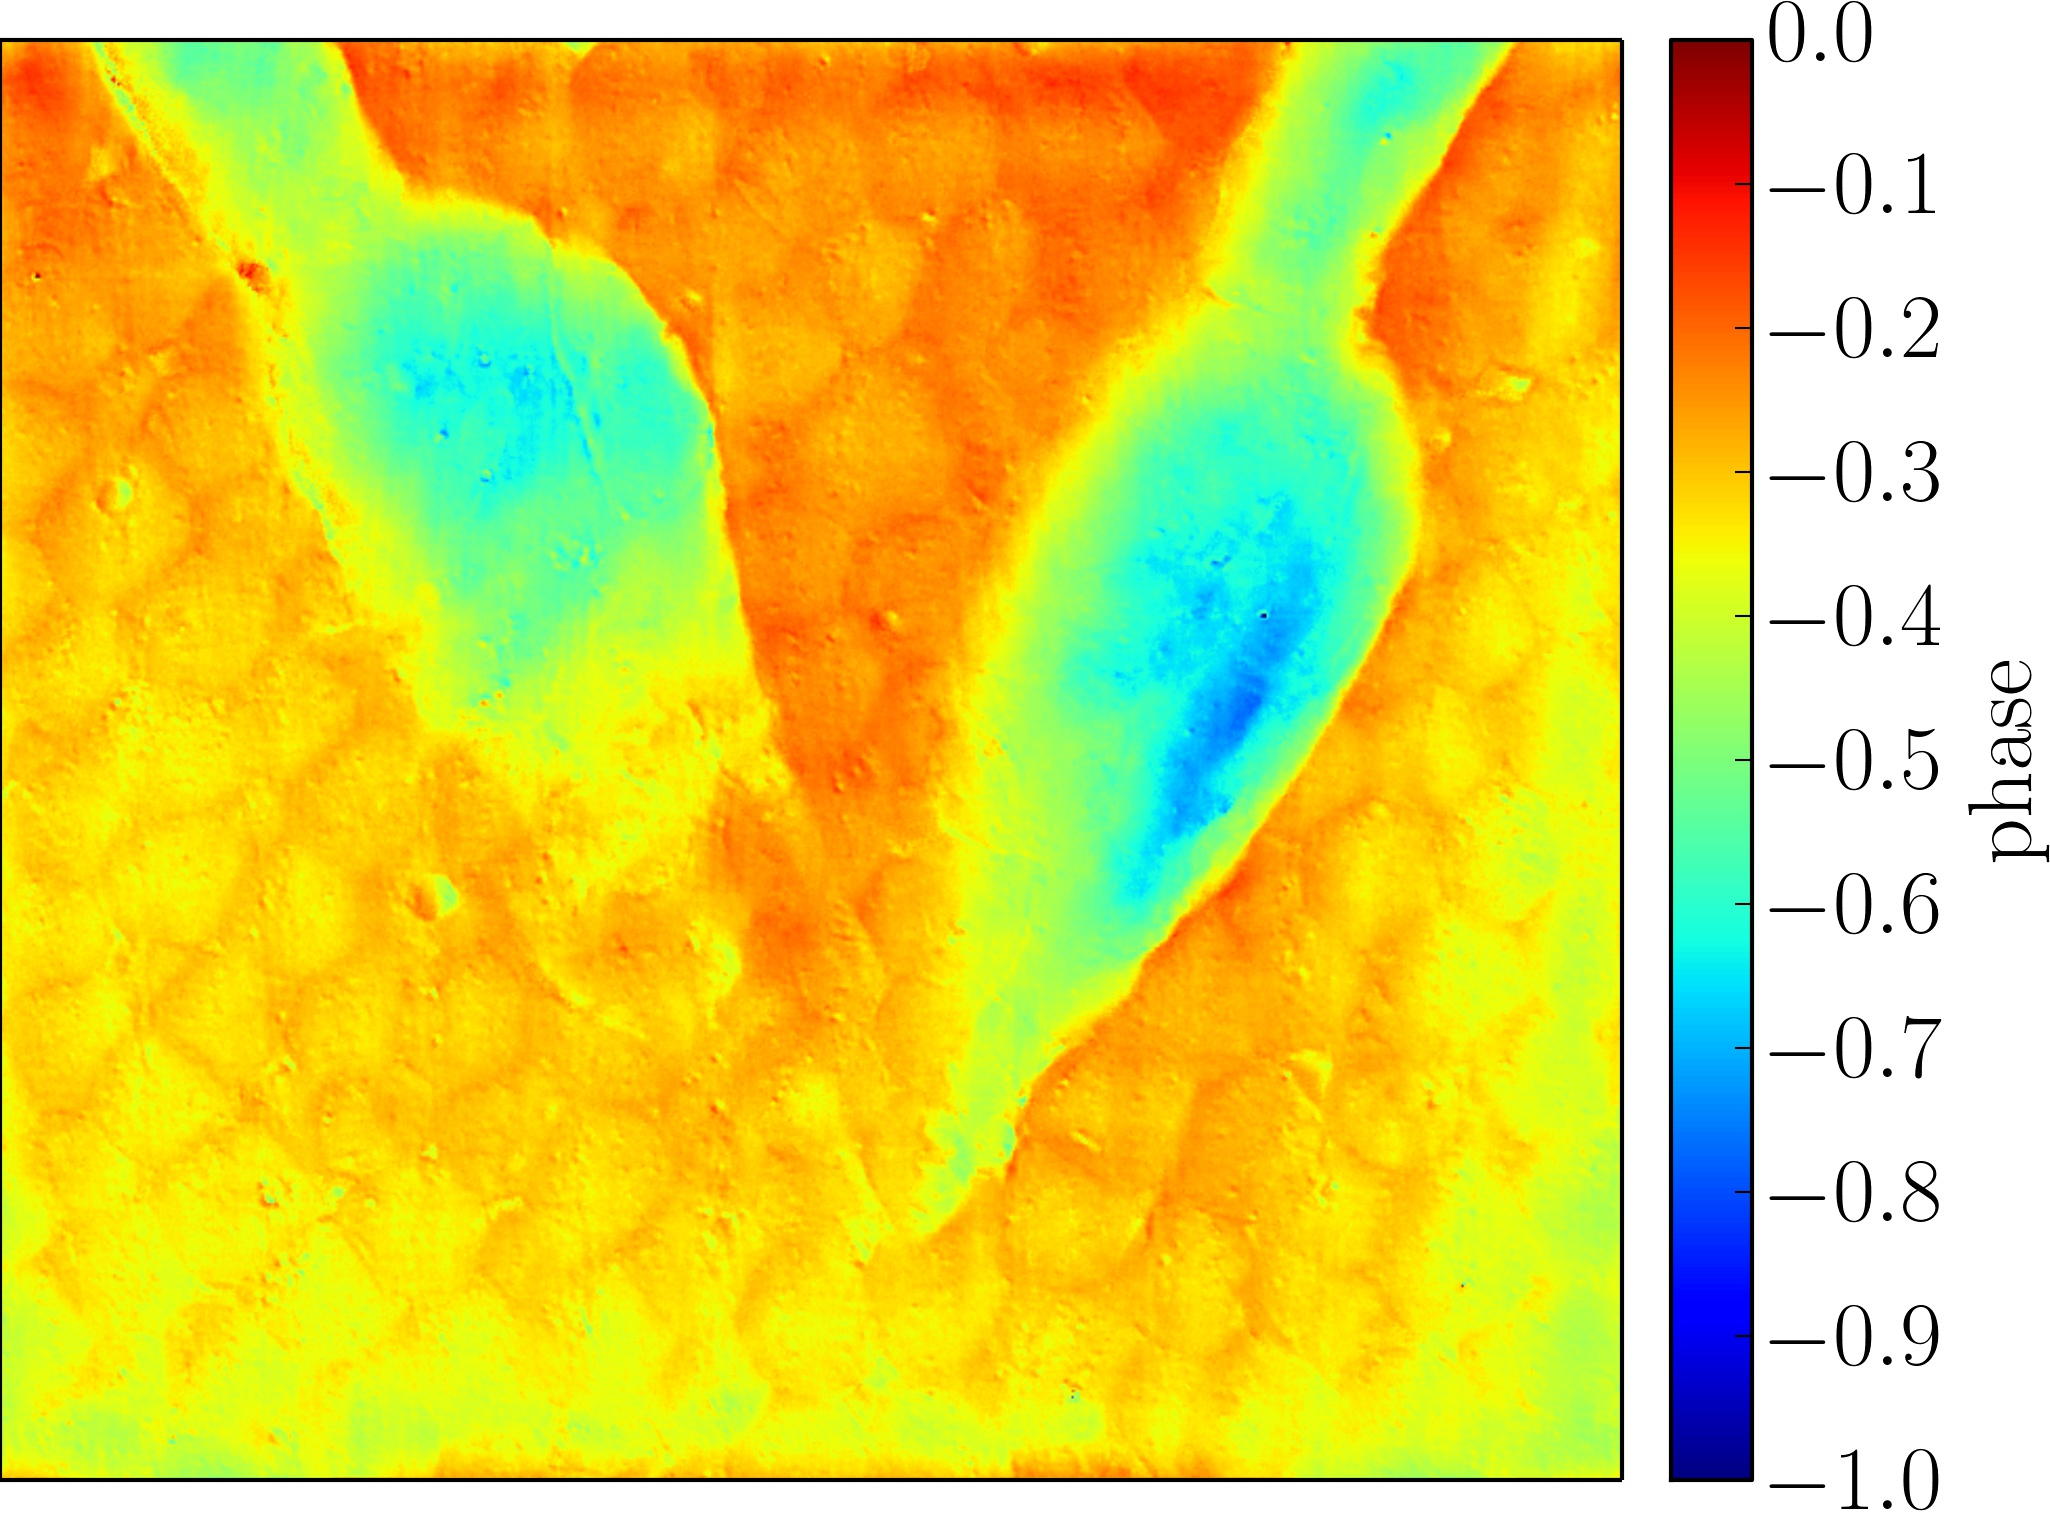
\includegraphics[width=0.4\textwidth]{figures/V_filtered.jpg}}
	\caption[Unprocessed and processed phase maps of styrofoam board with engraving]{Phase maps of the styrofoam board with engraving (a) unprocessed (b) after removal of vignetting effect through DBS, (c) after removal of fringe artifacts through FFT-filtering.}
	\label{fig:Vprocessed}
\end{figure}

\captionsetup[figure]{width=6.2in}
\begin{figure}[h!]
	\centering
	\subfigure[]{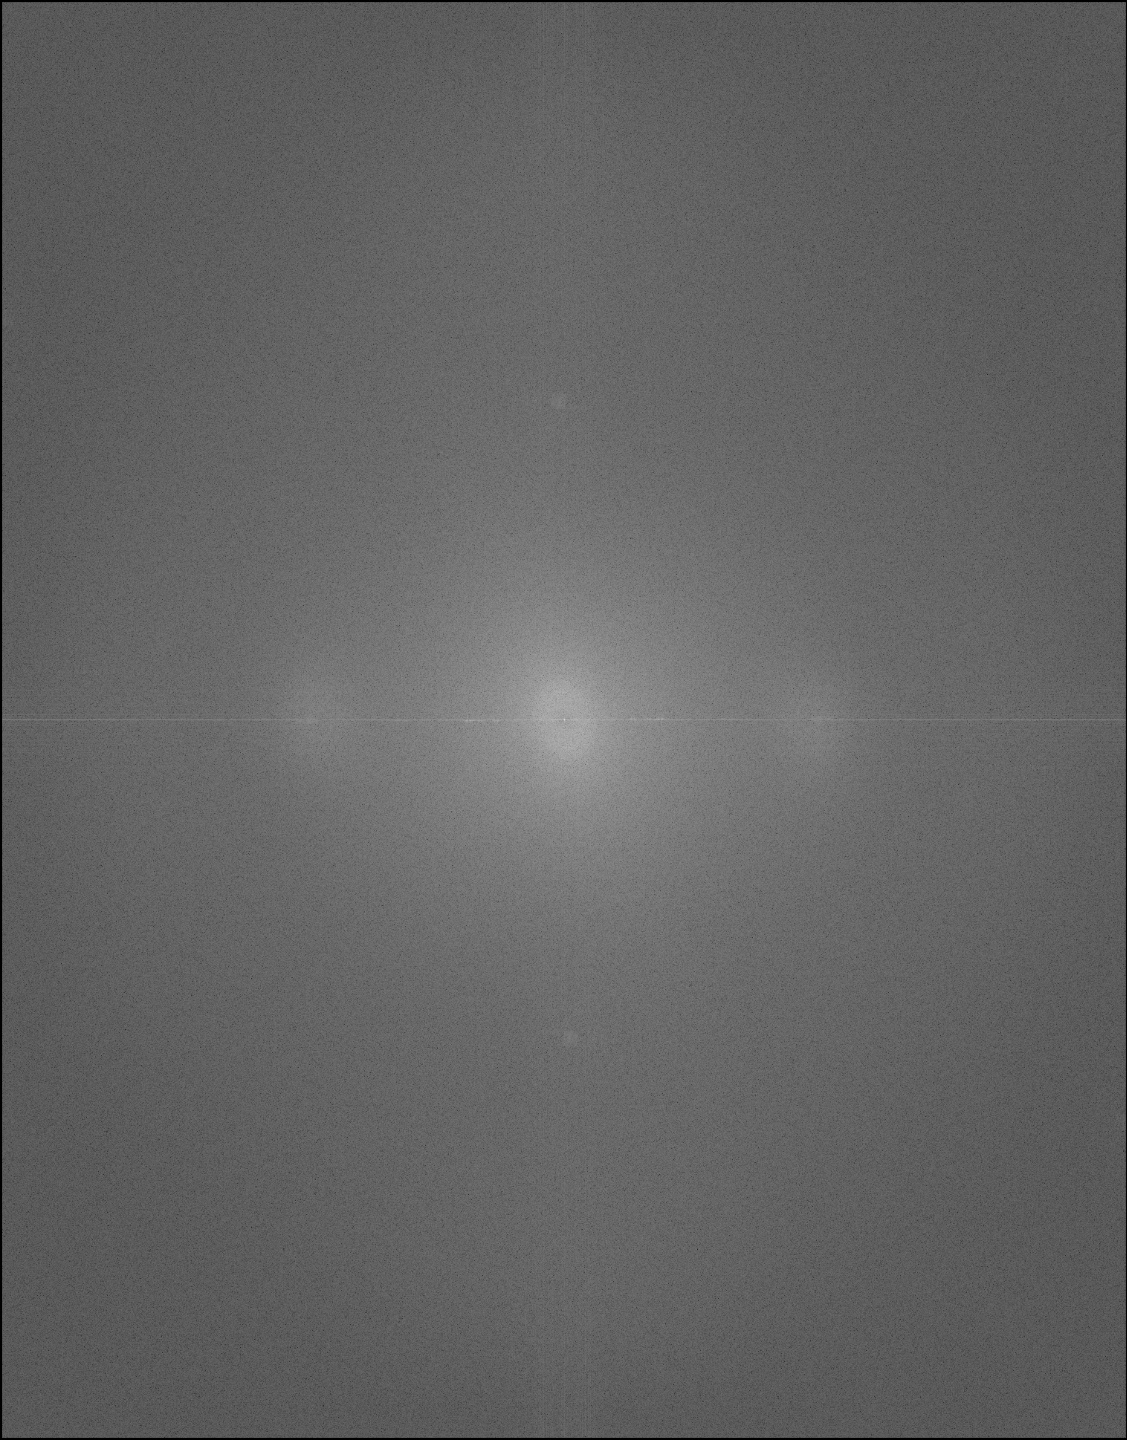
\includegraphics[width=0.3\textwidth]{figures/stone_fft.jpg}}
	\subfigure[]{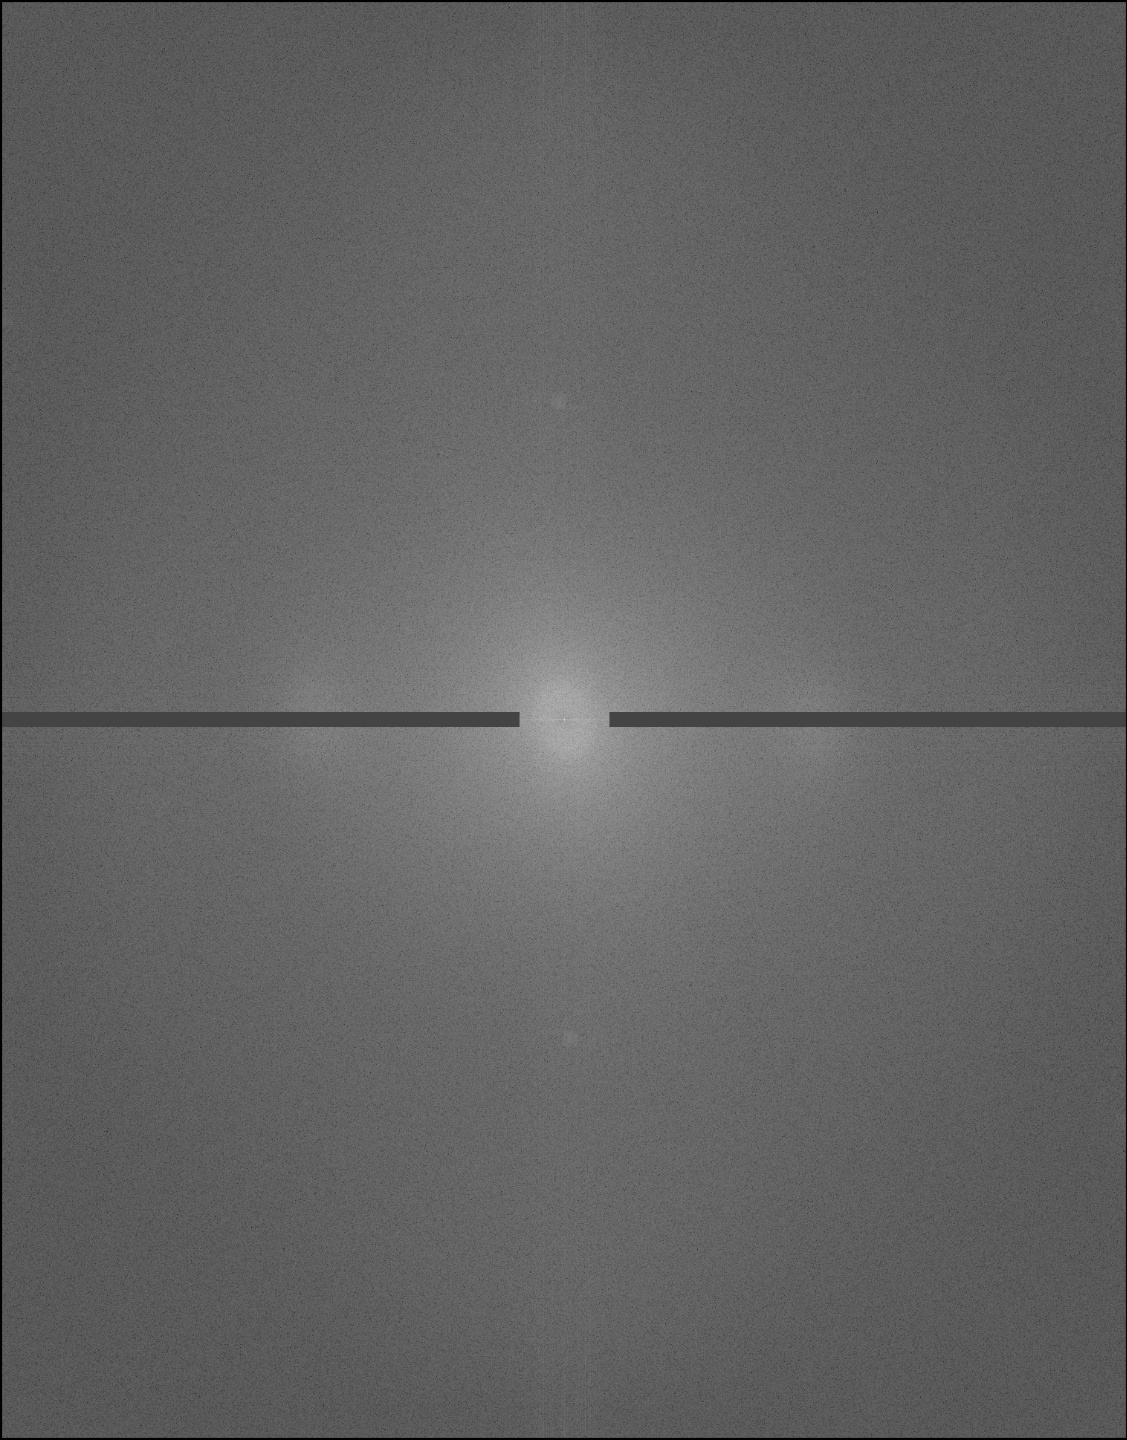
\includegraphics[width=0.3\textwidth]{figures/stone_mask.jpg}}
	\subfigure[]{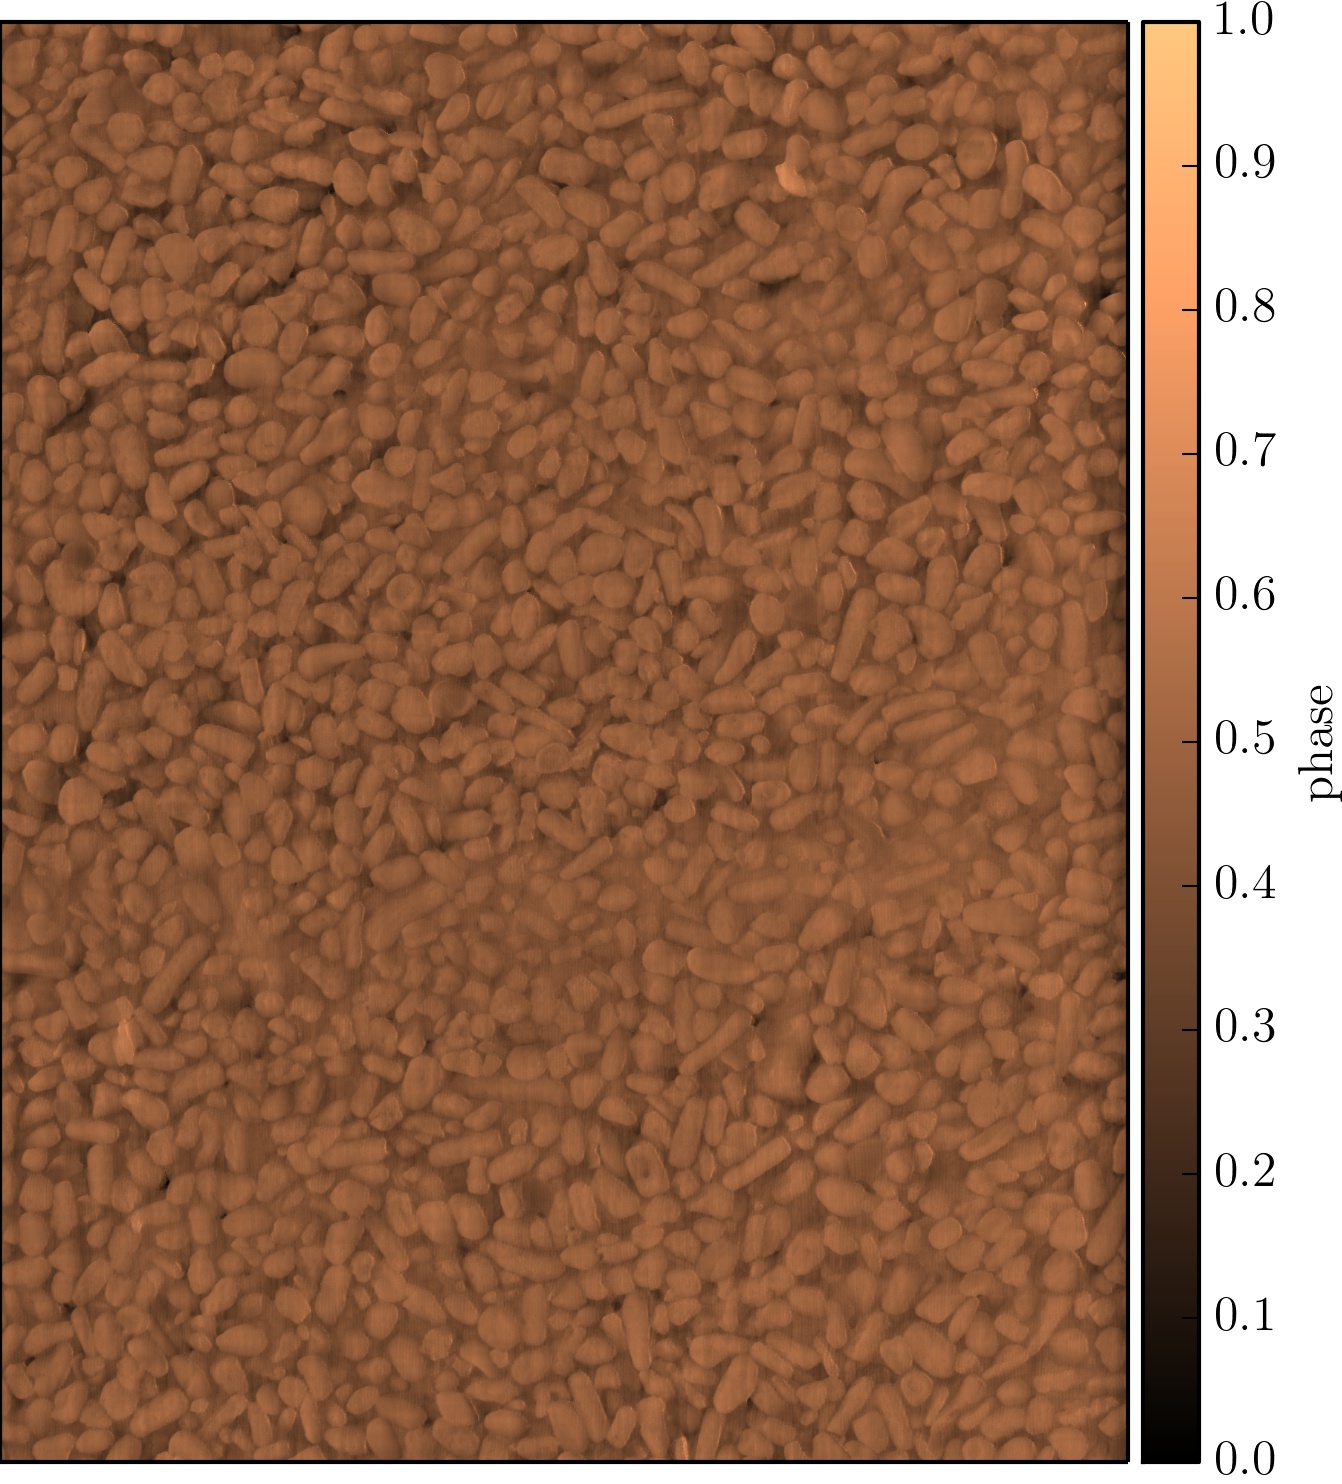
\includegraphics[width=0.35\textwidth]{figures/stonefinal.jpg}}
	\caption[FFT of pebbled wall]{Pebbled wall: (a) FFT, (b) filter mask, (c) phase map after filtering.}
	\label{fig:stonefft}
\end{figure}

The same procedure was followed for the processed (without vignetting effect) pebbled wall and step pyramid in Chapter 4. Shown in Figures \ref{fig:stonefft} and \ref{fig:pyramidfft} are their FFT's, filter masks, and phase map after filtering. 

The same peaks were observed for the pebbled wall. As for the pyramid, its edges may be seen as repeating lines so they have reduced sharpness after filtering. Hence, we reiterate that careful consideration of the filter mask must be made to only remove the unwanted fringes.

\begin{figure}[h!]
	\centering
	\subfigure[]{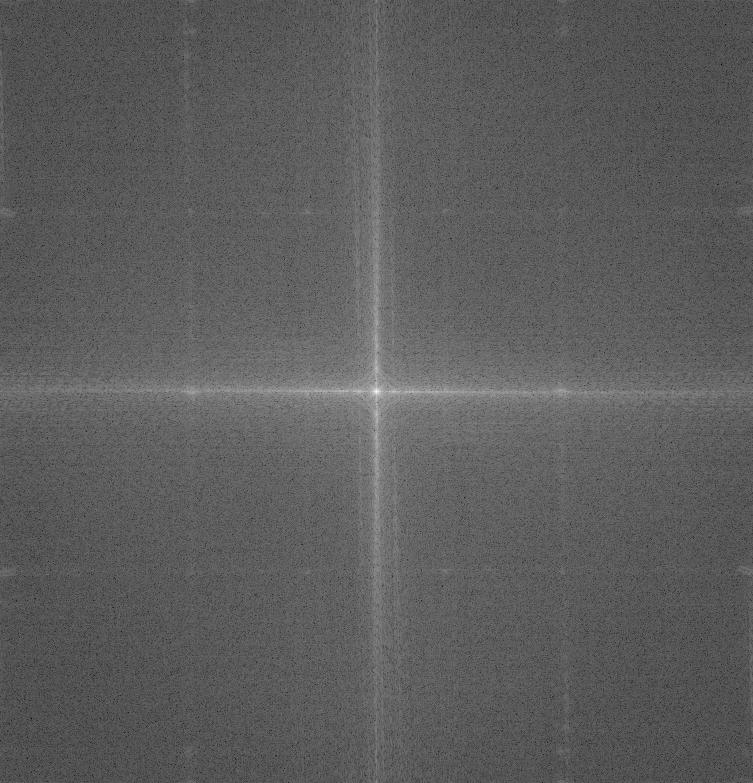
\includegraphics[width=0.3\textwidth]{figures/bigpyrfft.jpg}}
	\subfigure[]{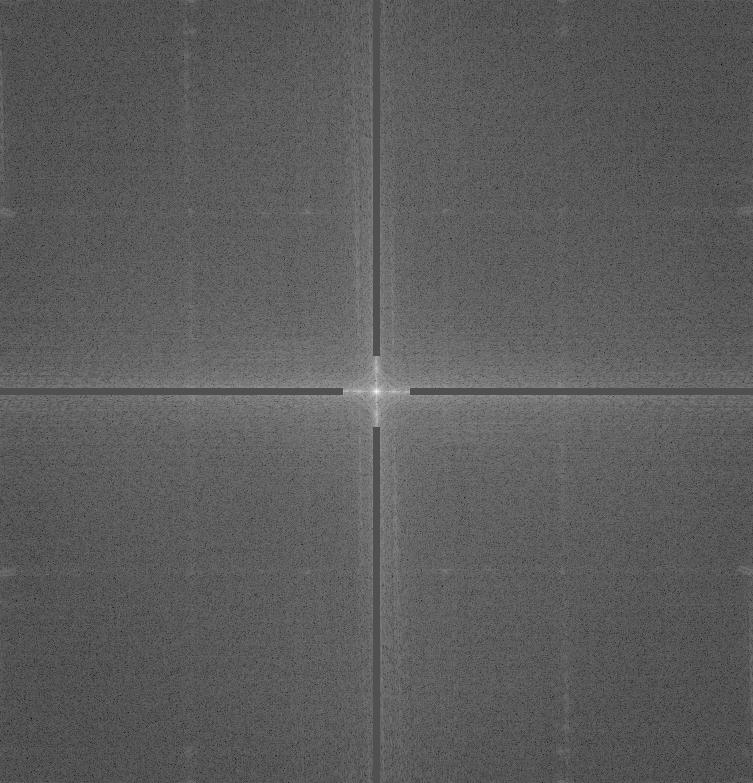
\includegraphics[width=0.3\textwidth]{figures/bigpyrmask.jpg}}
	\subfigure[]{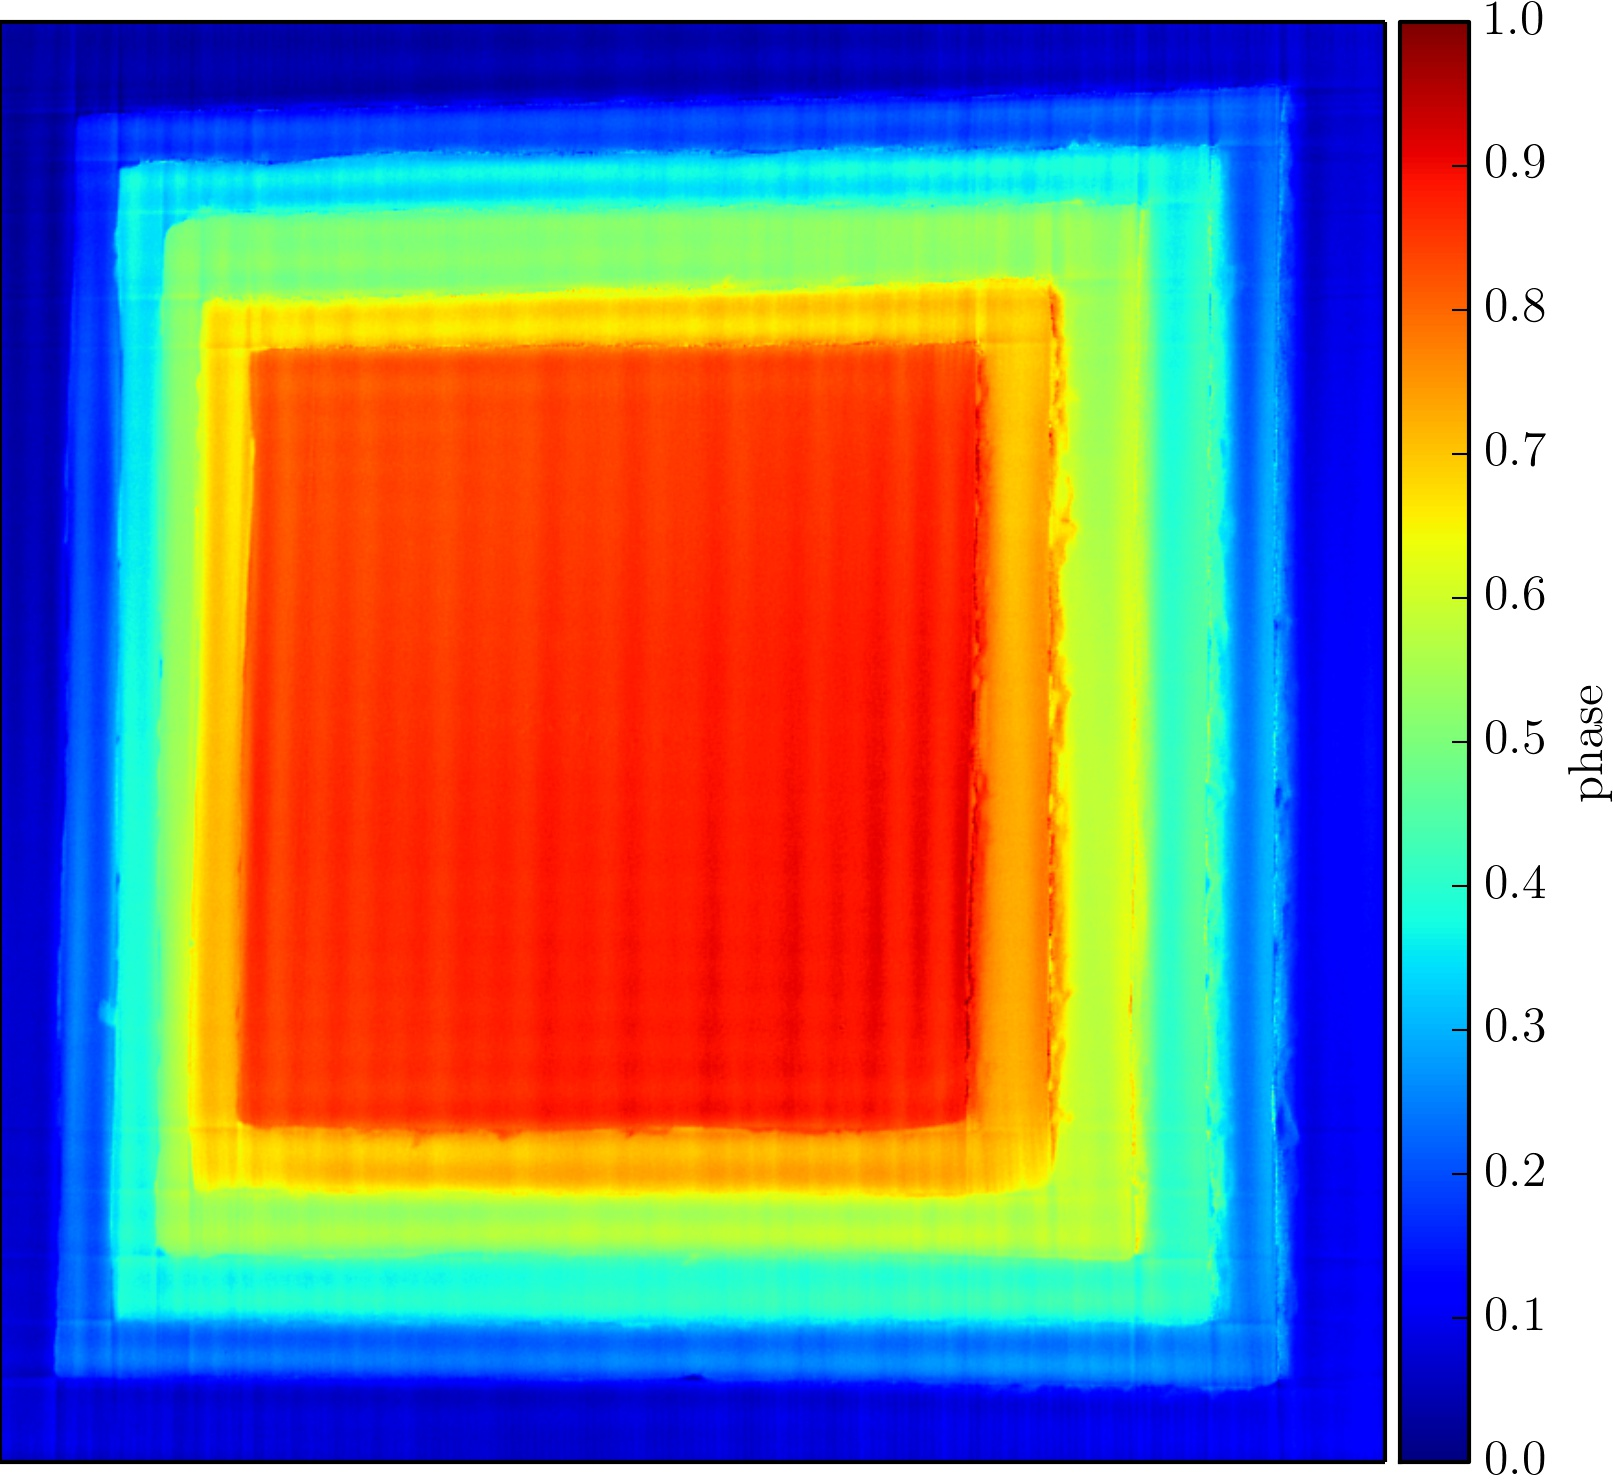
\includegraphics[width=0.33\textwidth]{figures/bigpyrfinal.jpg}}
	\caption[FFT of step pyramid]{Step pyramid: (a) FFT, (b) filter mask, (c) phase map after filtering.}
	\label{fig:pyramidfft}
\end{figure}
